\begin{Chapter}

\chapter{Title Example1}

\section{Equation}
To reference your equation, it should use the expressions such as "E.q.~\eqref{eq1}" or "Equation ~\eqref{eq1}".
\begin{equation} 
    \mbox{$x = \dfrac{-b\pm\sqrt{b^2-4ac}}{2a}$}
\end{equation}
\label{eq1}

\subsection{Table}

\text Content Text Content Text Content Text Content Text Content Text Content Text Content Text Content Text.

\begin{table*}[htbp]
    \centering
    \caption{Table Example AAA.} \label{tab: complexity1}
    \makebox[\linewidth][c]{
    \renewcommand\arraystretch{1.2}{
        \begin{tabular}{| l | c  c  c  c |}
        \hline
        Protocol & $P$ & $CS_1$ & $CS_2$ & $RG$ \\
        \hline
        SD & $O(1)$, $O(1)$, N/A & $O(n-t)$, $O(1)$, N/A & $O(n-t)$, $O(1)$, N/A & $O(1)$, $O(n)$, $O(n)$ \\
        MSSMul & $O(1)$, $O(1)$, N/A & $O(n-t)$, $O(n)$, $O(1)$ & $O(n-t)$, $O(n)$, N/A & $O(1)$, $O(n)$, $O(n)$ \\
        MSSAdd & $O(1)$, $O(1)$, N/A & $O(n-t)$, $O(n)$, $O(1)$ & N/A, N/A, N/A & $O(1)$, $O(n)$, $O(n)$ \\
        SC & $O(1)$, $O(1)$, N/A & $O(n-t)$, $O(n)$, $O(1)$ & $O(n-t)$, $O(n)$, N/A & $O(1)$, $O(n)$, $O(n)$ \\
        \hline 
        \end {tabular}
    }}
\end {table*}

\subsubsection{Section Header Level 3}

\begin{equation} 
    \mbox{$(1+x)^n = 1 + \dfrac{nx}{1!} + \dfrac{n(n-1)x^2}{2!}$}
\end{equation}

You can also make a little text or a number appear on other text or number, like this $10^{-4}$, or $10^{a}$, and $a^{-10}$. These are called "a power of a number", or \textit{exponent}, which indicates how many times a base number is multiplied by itself. Figure \ref{fig: image1} and Figure \ref{fig: image2} show the train station, and Table \ref{tab: complexity1} shows the table.

\begin{figure*}[htbp]
    \centering
    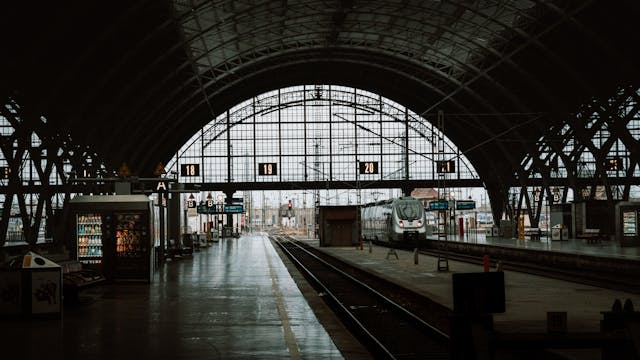
\includegraphics[width = 1\textwidth]{pics/image.jpeg}
    \caption{Cool train station}
    \label{fig: image1}
\end{figure*}

\begin{figure*}[htbp]
    \centering
    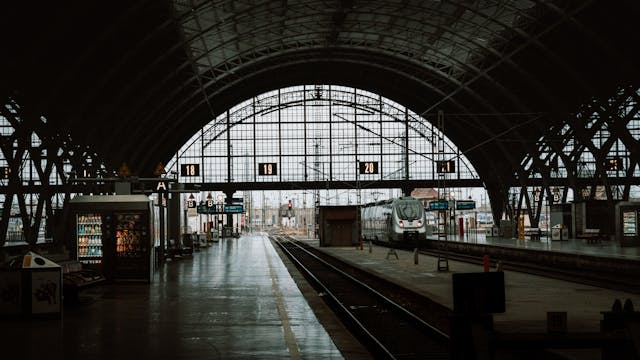
\includegraphics[width = 1\textwidth]{pics/image.jpeg}
    \caption{This cool train station stands as a metaphor for life itself, everyone's waiting, no one knows when their train will arrive, and someone's always holding the wrong ticket. Yet, we all stand here pretending everything's fine, sipping overpriced coffee with quiet determination}
    \label{fig: image2}
\end{figure*}

\begin{figure*}[htbp]
    \centering
    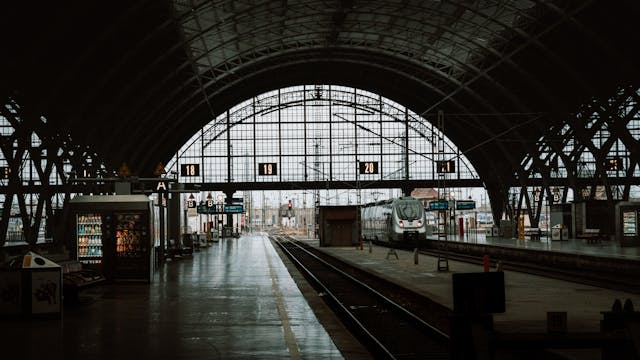
\includegraphics[width = 1\textwidth]{pics/image.jpeg}
    \caption{Cool train station}
    \label{fig: image2}
\end{figure*}

Content Text Content Text Content Text Content Text Content Text Content Text Content Text Content Text Content Text Content Text Content Text Content Text Content Text.

\begin{figure*}[htbp]
    \centering
    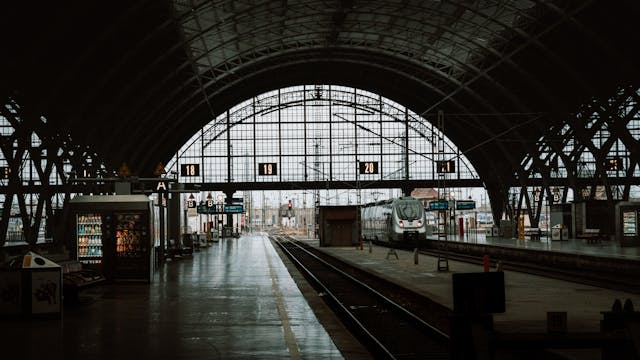
\includegraphics[width = 0.5\textwidth]{pics/image.jpeg}
    \caption{Cool train station}
    \label{fig: image}
\end{figure*}

\end{Chapter}